\begin{dang}{Đơn điệu hàm hợp, hàm chứa dấu giá trị tuyệt đối}
    \begin{itemize}
        \item Hàm $y=f(u)$.
        \begin{itemize}
            \item \textbf{Bước 1:} Tính đạo hàm $y'=u'\cdot f'(u)$.
            \item \textbf{Bước 2:} Lập bảng xét dấu của $y'$.
            \item \textbf{Bước 3:} Kết luận.
        \end{itemize}
        \item Hàm $y=f(u)+g(x)$.
        \begin{itemize}
            \item \textbf{Bước 1:} Tính đạo hàm $y'=u'f'(u)+g'(x)$.
            \item \textbf{Bước 2:} Lập bảng xét dấu của $y'$ (dựa vào tương giao giữa hai đồ thị).
            \item \textbf{Bước 3:} Kết luận.
        \end{itemize}
        \item Hàm $y=|f(x)|$.
        \begin{itemize}
            \item \textbf{Bước 1:} Lập bảng biến thiên hàm $y=f(x)$
            \item \textbf{Bước 2:} Lập bảng biến thiên hàm $y=|f(x)|$ từ hàm $y=f(x)$ bằng cách lấy đối xứng phần dưới trục $Ox$ qua trục $Ox$.
            \item \textbf{Bước 3:} Kết luận.
        \end{itemize}
    \end{itemize}
\end{dang}
\begin{vd}%[2D1K1-2]
    Cho hàm số $y=f(x)$ liên tục trên $\mathbb{R}$ có bảng xét dấu như hình vẽ
    \begin{center}
        
\begin{tikzpicture}
            \tkzTabInit[lgt=1,espcl=2.5,deltacl=0.6]
            {$x$ /0.6,$f'$ /0.6}
            {$-\infty$,$-1$,$0$,$1$,$+\infty$}
            \tkzTabLine{,-,$0$,+,$0$,-,$0$,+,}
        \end{tikzpicture}
    \end{center}
    Tìm các khoảng đơn điệu của hàm số sau
    \begin{listEX}[3]
        \item $y=f(4+3x)$.
        \item $y=f(5-2x)+3$.
        \item $y=f(2x^2-x)$.
        %	\item $y=f\left(f(x)\right)$, biết $f(x)>2,\forall x \in\mathbb{R}$.
    \end{listEX}
    \loigiai{\dotlineEX{42}}
\end{vd}
\begin{vd}%[2D1G1-2]
    \immini{	Cho hàm số $y=f(x)$ và đồ thị của hàm số $y=f'(x)$ như hình vẽ. 	Tìm các khoảng đơn điệu của hàm số sau
        \begin{listEX}[2]
            \item $y=f(x)+x$.
            \item $y=f(2x+1)+4x-3$.
            \item $y=f(x)-x^2$.
            \item $y=f(2x+1)-2x^2+6x+1$
    \end{listEX}}{\begin{tikzpicture}[>=stealth,y=.7cm,font=\footnotesize]
            \def\a{1}
            \path
            (0,0) coordinate (O)
            (-1,0) coordinate (A)node[above]{$ -1 $}
            (1,0) coordinate (B)node[below]{$ 1 $}
            (0,-1) coordinate (C)node[right]{$ -2 $}
            (0,1) coordinate (D)node[left]{$ 2 $}
            %	Các điểm mút cho lệnh controls:
            (-1,-1) coordinate (P)
            (-0.3,0.5) coordinate (N)
            (0.3,-0.5) coordinate (Q)
            (1,1) coordinate (M)
            ;
            %Vẽ đường cong, đường thẳng:
            %	\draw[red] (P)--(N)--(Q)--(M);
            \draw[name path=fx,shorten >=-1cm, shorten <=-0.5cm] (P)..controls +(75:0.5) and +(185:0.25)..(N)..controls +(-10:0.3) and +(170:0.3)..(Q)..controls +(2:0.35) and +(-105:0.25)..(M);
            %Vẽ hệ trục tọa dộ:
            \draw[->] (-1.5,0)--(0,0) node[below left]{$O$}--(2,0) node[below]{$x$};
            \draw[->] (0,-1.5) --(0,2.35) node[left]{$y$};
            %-2,-1,1,2,3
            \draw[dashed](B)|-(D) (A)|-(C);
            \foreach \p in {M,P,O,A,B,C,D}
            \fill (\p) circle (1pt);
    \end{tikzpicture}}
    \loigiai{}
\end{vd}
\begin{vd}%[2D1G1-3]
    Cho hàm số $y=f(x)$ liên tục trên $\mathbb{R}$ có đồ thị hàm $y=f'(x)$ như hình vẽ.
    \begin{center}
        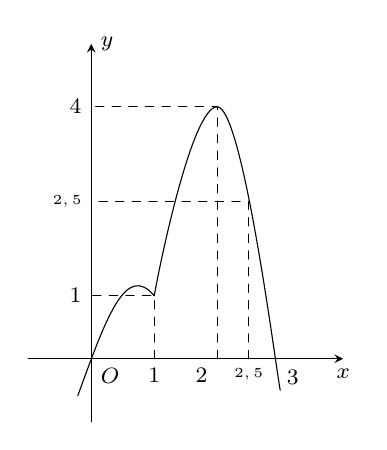
\begin{tikzpicture}[>=stealth, line join=round, line cap=round, font=\footnotesize, scale=.8]
            \draw[<->] (4,0)node[below]{$x$}-|(0,5)node[right]{$y$};
            \draw (-1,0)-|(0,-1)
            (0,0)node[below right]{$O$};
            \draw node at (3.2,-0.3) {$3$};
            \draw[dashed] (1,0)node[below]{$1$}|-(0,1)node[left]{$1$}
            (2,0)node[below left]{$2$}|-(0,4)node[left]{$4$} (2.5,0)node[below]{\tiny $2,5$}|-(0,2.5)node[left]{\tiny $2,5$}
            ;
            \draw[shorten <= -.5cm]
            (0,0) ..controls +(70:.7) and +(130:.7) ..
            (1,1) ..controls +(80:.5) and +(180:.4) ..
            (2,4) ..controls +(0:.4) and +(100:.5) .. (3,-.5)
            ;
        \end{tikzpicture}
    \end{center}
    \begin{listEX}
        \item Tìm các khoảng nghịch biến của hàm số $g(x)=|f(-x^4+2x^3-x^2+1)|$, biết$f(3)<0$.
        \item Tìm các khoảng đồng biến của hàm số $h(x)=|3f(x)-x^3|$, biết $f(0)=0$.
        \item Tìm $m$ để hàm số $y=|3f(x)-x^3+m|$ nghịch biến trên $(0;2)$, biết $f(2)=1$.
        \item Tìm $a$ để hàm số $y=|4f(\sin x)+\cos 2x-a|$ nghịch biến trên $\left(0;\dfrac{\pi}{2}\right)$, biết $f(1)=1$.
    \end{listEX}
    \loigiai{\dotlineEX{25}}
\end{vd}
\BTTN
\Opensolutionfile{ans}[ans/2D1-1-DANG-3]
\begin{ex}%[2D1G1-2]
    Cho hàm số có đạo hàm liên tục trên $\mathbb{R}$, dấu của đạo hàm được cho bởi bảng dưới đây:
    \begin{center}
        
\begin{tikzpicture}
            \tkzTabInit[lgt=1.2,espcl=2.5,deltacl=.5]
            {$x$ /.7, $f'(x)$ /.7}
            {$-\infty$,$0$,$2$,$+\infty$}
            \tkzTabLine{,+,$0$,-,$0$,+,}
            %\tkzTabVar{+/$+\infty$,-/$-3$,+/$-\infty$}
        \end{tikzpicture}
    \end{center}
    Hàm số $g(x)=f(2x-2)$ nghịch biến trong khoảng nào dưới đây?
    \choice
    {$(-1;1)$}
    {$(2;+\infty)$}
    {\True $(1;2)$}
    {$(-\infty;-1)$}
    \loigiai{
        Ta có $g(x)=f(2x-2)\Rightarrow g'(x)=2f'(2x-2)$.
        \\
        Theo bảng xét dấu của đạo hàm ta có $f'(x)<0 \Leftrightarrow 0<x<2$.
        \\
        Nên $f'(2x-2)<0 \Leftrightarrow 0<2x-2<2 \Leftrightarrow 1<x<2$.
        \\
        Vậy hàm số $g(x)=f(2x-2)$ nghịch biến trên khoảng $(1;2)$.
    }
\end{ex}
\begin{ex}%[2D1K1-2]
    Cho hàm số $f(x)$ có bảng xét dấu đạo hàm như hình bên dưới
    \begin{center}
        
\begin{tikzpicture}
            \tkzTabInit[lgt=1.2,espcl=2.5]
            {$x$ /.7, $y'$ /.7}
            {$-\infty$,$-1$,$6$,$+\infty$}
            \tkzTabLine{ ,+,$0$,-,$0$, +, }
        \end{tikzpicture}
    \end{center}
    Hàm số $y=f(2-x)$ đồng biến trên khoảng
    \choice
    {$\left(-3;4\right)$}
    {$\left(-1;6\right)$}
    {\True $\left(-4;3\right)$}
    {$\left(3;+\infty \right)$}
    \loigiai{
        Ta có $y'=-f'(2-x)$, $y'=0 \Leftrightarrow \hoac{&2-x=-1\\&2-x=6} \Leftrightarrow \hoac{&x=3\\&x=-4.}$\\
        Ta có bảng xét dấu
        \begin{center}
            
\begin{tikzpicture}
                \tkzTabInit[lgt=1.2,espcl=2.5]
                {$x$ /1, $y'$ /1}
                {$-\infty$,$-4$,$3$,$+\infty$}
                \tkzTabLine{ ,-,$0$,+,$0$, -, }
            \end{tikzpicture}
        \end{center}
        Vậy hàm số nghịch biến trên khoảng $(-4;3)$.
    }
\end{ex}
\begin{ex}%[2D1K1-2]
    Cho hàm số $f(x)$ có bảng xét dấu đạo hàm như hình bên dưới
    \begin{center}
        
\begin{tikzpicture}
            \tkzTabInit[lgt=1.2,espcl=2.5]
            {$x$ /.7, $y'$ /.7}
            {$-\infty$,$1$,$5$,$+\infty$}
            \tkzTabLine{ ,-,$0$,+,$0$, -, }
        \end{tikzpicture}
    \end{center}
    Hàm số $y=f(1-2x)+3$ nghịch biến trên khoảng
    \choice
    {$\left(1;3\right)$}
    {\True $\left(-2;0\right)$}
    {$\left(-\infty;1\right)$}
    {$\left(5;+\infty \right)$}
    \loigiai{
        Ta có $y'=-2f'(1-2x)$, $y'=0 \Leftrightarrow \hoac{&1-2x=1\\&1-2x=5} \Leftrightarrow \hoac{&x=0\\&x=-2.}$\\
        Ta có bảng xét dấu
        \begin{center}
            
\begin{tikzpicture}
                \tkzTabInit[lgt=1.2,espcl=3]
                {$x$ /1, $y'$ /1}
                {$-\infty$,$-2$,$0$,$+\infty$}
                \tkzTabLine{ ,+,$0$,-,$0$, +, }
            \end{tikzpicture}
        \end{center}
        Vậy hàm số nghịch biến trên khoảng $(-2;0)$.
    }
\end{ex}
\begin{ex}%[2D1G1-2]
    \immini{Cho hàm số $y=f(x)$. Hàm số $y=f'(x)$ có đồ thị như hình bên. Hàm số $y=f(2-x)$ đồng biến trên khoảng nào dưới đây?
        \choice
        {$(1;3)$}
        {$(2;+\infty)$}
        {\True $(-2;1)$}
        {$(3;+\infty)$}
    }
    {
        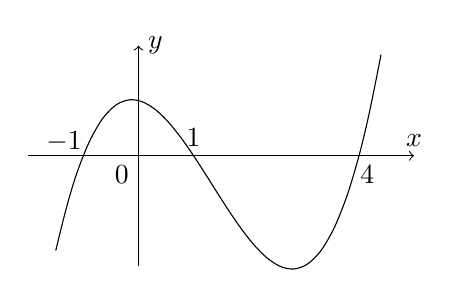
\begin{tikzpicture}[scale=0.7]
            \def\xmin{-2} \def\xmax{5} \def\ymin{-2} \def\ymax{2}
            \draw [->](\xmin,0)--(\xmax,0) node [above]{$x$};
            \draw [->](0,\ymin)--(0,\ymax) node [right]{$y$};
            \draw (0,0) node [below left]{$0$};
            \draw plot[smooth,tension=0.7,domain=-1.5:4.4,line width=1pt] (\x,{0.25*(\x)^3-(\x)^2-0.25*\x+1});
            \draw (-1,0) node [above,xshift=-7pt,yshift=-2pt]{$-1$};
            \draw (1,0) node [above]{$1$} (4,0) node [below,xshift=3pt]{$4$};
        \end{tikzpicture}
    }
    \loigiai{
        Ta có $y=f(2-x) \Rightarrow y'=-2f(2-x)$.
        \\
        Hàm số $y=f(2-x)$ đồng biến ta cần có $y'>0$
        \\
        $\Leftrightarrow f'(2-x)<0 \Leftrightarrow \hoac{&2-x<-1\\&1<2-x<4}\Leftrightarrow \hoac{&x>3\\&-2<x<1.}$
    }
\end{ex}
\begin{ex}%[2D1K1-2]
    \immini{
        Cho hàm số $y=f(x)$ có đạo hàm liên tục trên $\mathbb{R}$. Biết đồ thị hàm số $y=f'(x)$ chỉ cắt trục hoành tại $3$ điểm như hình bên. 	Hàm số $y=f(2x+5)+1$ đồng biến trên khoảng
        \choice
        {$\left(-3;-2\right)$}
        {\True $\left(-2;-1\right)$}
        {$\left(-1;1\right)$}
        {$\left(-3;+\infty\right)$}
    }{
        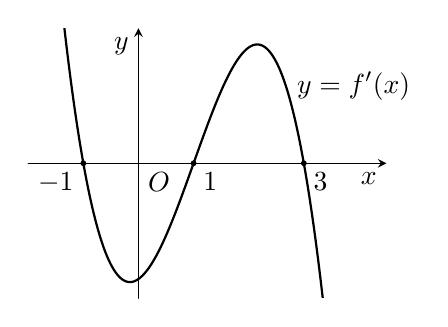
\begin{tikzpicture}[scale=0.7,y=.7cm,line join=round, line cap=round,>=stealth]
            \tikzset{label style/.style={font=\footnotesize}}
            %%Nhập giới hạn đồ thị và hàm số cần vẽ
            \def \xmin{-2}
            \def \xmax{4.5}
            \def \ymin{-3.5}
            \def \ymax{3.5}
            \draw[->] (\xmin,0)--(\xmax,0) node[below left] {$x$};
            \draw[->] (0,\ymin)--(0,\ymax) node[below left] {$y$};
            \draw (0,0) node [below right] {$O$};
            \node[below right] at (1,0) {$1$};
            \node[below right] at (3,0) {$3$};
            \node[below left] at (-1,0) {$-1$};
            \node[right] at (2.7,2) {$y=f'(x)$};
            \foreach \i in {-1,1,3} \draw[fill=black] (\i,0) circle(1.2pt);
            \begin{scope}
                \clip (\xmin+0.01,\ymin+0.01) rectangle (\xmax-0.01,\ymax-0.01);
                \draw[samples=350,domain=\xmin+0.01:\xmax-0.01,smooth,thick] plot (\x,{-(\x+1)*(\x-1)*(\x-3)});
            \end{scope}
        \end{tikzpicture}
    }
    \loigiai{
        Ta có bảng xét dấu của $f'(x)$
        \begin{center}
            
\begin{tikzpicture}
                \tkzTabInit[lgt=1.2,espcl=3]
                {$x$ /1, $f'(x)$ /1}
                {$-\infty$,$-1$,$1$,$3$,$+\infty$}
                \tkzTabLine{ ,+,$0$,-,$0$,+,$0$, -, }
            \end{tikzpicture}
        \end{center}
        Ta có $y'=2f'(2x+5)$, $y'=0 \Leftrightarrow \hoac{&2x+5=-1\\&2x+5=1\\&2x+5=3} \Leftrightarrow \hoac{&x=-3\\&x=-2\\&x=-1.}$\\
        Ta có bảng xét dấu
        \begin{center}
            
\begin{tikzpicture}
                \tkzTabInit[lgt=3.2,espcl=3]
                {$x$ /1, $y'=2f'(2x+5)$ /1}
                {$-\infty$,$-3$,$-2$,$-1$,$+\infty$}
                \tkzTabLine{ ,+,$0$,-,$0$,+,$0$, -, }
            \end{tikzpicture}
        \end{center}
        Vậy hàm số đồng biến trên khoảng $\left(-\infty;-3\right)$ và $\left(-2;-1\right)$.
    }
\end{ex}
\begin{ex}%[2D1K1-2]
    \immini{Cho hàm số $y=f(x)$ có đạo hàm liên tục trên $\mathbb{R}$. Biết đồ thị hàm số $y=f'(x)$ chỉ cắt trục hoành tại $3$ điểm như hình bên dưới. Hàm số $y=f(1-3x)-4$ nghịch biến trên khoảng
        \choice
        {$\left(-\dfrac{1}{3};\dfrac{1}{3}\right)$}
        {\True $\left(\dfrac{1}{3};\dfrac{2}{3}\right)$}
        {$\left(0;2\right)$}
        {$\left(-\infty;0\right)$}
    }
    {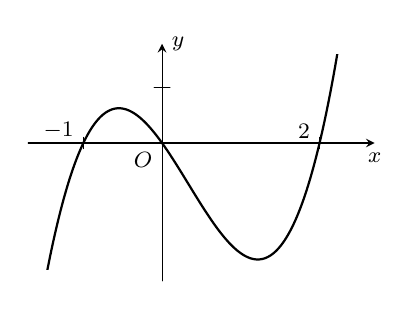
\begin{tikzpicture}[scale=1,y=.7cm, font=\footnotesize, line join=round, line cap=round, >=stealth]
            \def\xmin{-1.5}\def\xmax{2.5}\def\ymin{-2.3}\def\ymax{1.6}
            \draw[->] (\xmin-0.2,0)--(\xmax+0.2,0) node[below] {\footnotesize $x$};
            \draw[->] (0,\ymin-0.2)--(0,\ymax+0.2) node[right] {\footnotesize $y$};
            \draw (0,0) node [below left] {\footnotesize $O$};
            \foreach \x in {-1,2}\draw (\x,0.1)--(\x,-0.1) node [above left] {\footnotesize $\x$};
            \foreach \y in { }\draw (0.1,\y)--(-0.1,\y) node [left] {\footnotesize $\y$};
            \clip (\xmin,\ymin) rectangle (\xmax,\ymax);
            \draw[smooth,samples=200,domain=\xmin:\xmax,thick] plot (\x,{1*((\x)^3)+-1*((\x)^2)+-2*(\x)+0});
    \end{tikzpicture} }
    \loigiai{Ta có $y'=-3f'(1-3x)$. Khi đó $y'<0 \Leftrightarrow -3f'(1-3x)<0 \Leftrightarrow f'(1-3x)>0.$\\
        Dựa vào đồ thị hàm số ta có
        \[f'(1-3x)>0 \Leftrightarrow \hoac{&-1<1-3x<0\\&1-3x>2} \Leftrightarrow \hoac{&\dfrac{1}{3}<x<\dfrac{2}{3}\\& x<-\dfrac{1}{3}.}\]
        Vậy hàm số nghịch biến $\left(\dfrac{1}{3};\dfrac{2}{3}\right)$.
    }
\end{ex}
\begin{ex}%[2D1G1-2]
    \immini{	Cho hàm số $f(x)$. Hàm số $f'(x)$ có đồ thị bên.
        Hàm số $y=f(1-2x)+x^2-x$ nghịch biến trên khoảng nào dưới đây?
        \choice
        {\True $\left(1; \dfrac{3}{2}\right)$}
        {$\left(0; \dfrac{1}{2}\right)$}
        {$\left(-2;-1\right)$}
        {$\left(2;3\right)$}
    }
    {
        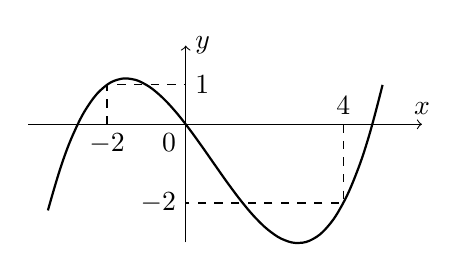
\begin{tikzpicture}[scale=0.5]
            \def\xmin{-4} \def\xmax{6} \def\ymin{-3} \def\ymax{2}
            \draw [->](\xmin,0)--(\xmax,0) node [above]{$x$};
            \draw [->](0,\ymin)--(0,\ymax) node [right]{$y$};
            \draw (0,0) node [below left]{$0$};
            %\clip (\xmin,\ymin) rectangle (\xmax,\ymax);
            \draw [thick]plot[smooth,tension=0.7,domain=-3.5:5,thick] (\x,{0.1*(\x)^3-0.2*(\x)^2-1.3*\x});
            \draw [dashed](-2,0) node[below] {$-2$}|-(0,1) node[right]{$1$} (4,0) node [above]{$4$}|-(0,-2) node [left]{$-2$};
        \end{tikzpicture}
    }
    \loigiai{
        Ta có $y=f(1-2x)+x^2-x \Rightarrow y'=-2f'(1-2x)+2x-1$.
        \\
        Để hàm số nghịch biến ta cần có $y'<0$
        \\
        $\Leftrightarrow -2f'(1-2x)+2x-1<0 \Leftrightarrow f'(1-2x)>-\dfrac{1-2x}{2}$.
        \\
        Đặt $t=1-2x$ ta có đồ thị của hàm số $y=f(t)$ và $y=-\dfrac{t}{2}$.
        \begin{center}
            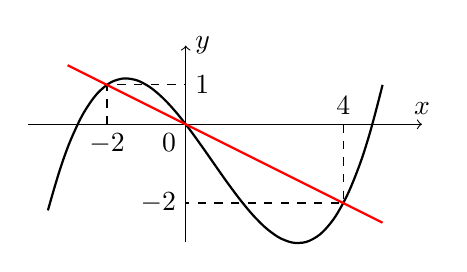
\begin{tikzpicture}[scale=0.5]
                \def\xmin{-4} \def\xmax{6} \def\ymin{-3} \def\ymax{2}
                \draw [->](\xmin,0)--(\xmax,0) node [above]{$x$};
                \draw [->](0,\ymin)--(0,\ymax) node [right]{$y$};
                \draw (0,0) node [below left]{$0$};
                %\clip (\xmin,\ymin-0.2) rectangle (\xmax,\ymax);
                \draw [thick]plot[smooth,tension=0.7,domain=-3.5:5] (\x,{0.1*(\x)^3-0.2*(\x)^2-1.3*\x});
                \draw [dashed](-2,0) node[below] {$-2$}|-(0,1) node[right]{$1$} (4,0) node [above]{$4$}|-(0,-2) node [left]{$-2$};
                \draw [thick, red](-3,1.5)--(5,-2.5);
            \end{tikzpicture}
        \end{center}
        Trên đoạn $[-2;4]$ thì $f(t)>\dfrac{t}{2} \Leftrightarrow -2<t<0$
        $\Leftrightarrow -2<1-2x<0 \Leftrightarrow \dfrac{1}{2}<x<\dfrac{3}{2}$.
        \\
        Vậy hàm số đồng biến trên khoảng $\left(1; \dfrac{3}{2}\right) \subset \left(\dfrac{1}{2}; \dfrac{3}{2}\right) $.
    }
\end{ex}
\begin{ex}%[2D1G1-2]
    \immini{Cho hàm số $y=f(x)$ có đạo hàm liên tục trên $\mathbb{R}$. Đồ thị hàm số $y=f'(3x+5)$ như hình vẽ.
        Hàm số $y=f(x)$ nghịch biến trên khoảng nào dưới đây?
        \choice
        {$\left(-\dfrac{7}{3};+\infty\right)$}
        {$\left(-\infty;10\right)$}
        {$\left(\dfrac{4}{3};+\infty\right)$}
        {\True $\left(-\infty;8\right)$}
    }
    {
        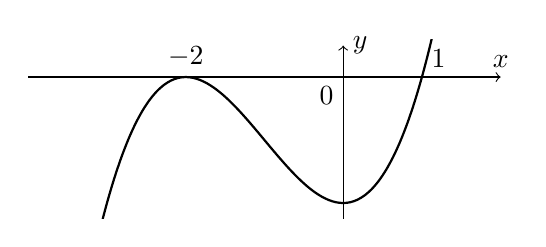
\begin{tikzpicture}[yscale=0.4]
            \def\xmin{-4} \def\xmax{2} \def\ymin{-4.5} \def\ymax{1}
            \draw [->](\xmin,0)--(\xmax,0) node [above]{$x$};
            \draw [->](0,\ymin)--(0,\ymax) node [right]{$y$};
            \draw (0,0) node [below left]{$0$};
            \clip (\xmin,\ymin) rectangle (\xmax+0.2,\ymax+0.2);
            \draw [thick]plot[smooth,samples=100,domain=-4:5] (\x,{(\x)^3+3*(\x)^2-4});
            \draw (-2,0) node [above]{$-2$} (1,0) node [above right]{$1$};
        \end{tikzpicture}
    }
    \loigiai{
        Đặt $x=3t+5$ ta có $g(t)=f(3t+5)\Rightarrow g'(t)=3f'(3t+5)$.
        \\
        $g'(t)<0 \Leftrightarrow f'(3t+5)<0\Leftrightarrow t<1$.
        \\
        Khi đó $f'(x)<0 \Leftrightarrow \dfrac{x-5}{3}<1 \Leftrightarrow x<8$.
    }
\end{ex}
\begin{ex}%[2D1G1-2]
    Cho đồ thị hàm số $y=f'(2-x^3)$ như hình vẽ.
    \immini{
        Hàm số $y=f(x)-x-1$ nghịch biến trong khoảng nào dưới đây?
        \choice
        {$(1;2)$}
        {$(2;+\infty)$}
        {$(-\infty;1)$}
        {\True $(-4;-1)$}
    }
    {
        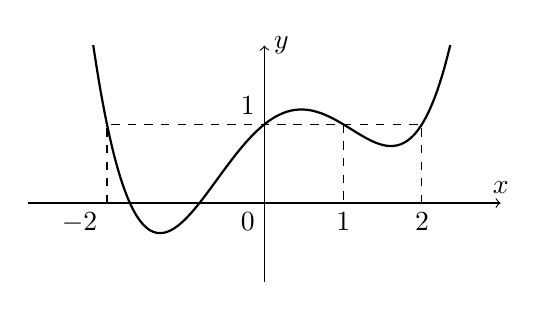
\begin{tikzpicture}
            \def\xmin{-3} \def\xmax{3} \def\ymin{-1} \def\ymax{2}
            \draw [->](\xmin,0)--(\xmax,0) node [above]{$x$};
            \draw [->](0,\ymin)--(0,\ymax) node [right]{$y$};
            \draw (0,0) node [below left]{$0$};
            \clip (\xmin,\ymin) rectangle (\xmax,\ymax);
            \draw [thick]plot[smooth,samples=100,domain=-4:5] (\x,{0.2*(\x)^4-0.2*(\x)^3-0.8*(\x)^2+0.8*\x+1});
            \draw (-2,0) node [below left]{$-2$} (1,0) node [below]{$1$} (2,0) node [below]{$2$};
            \draw [dashed](-2,0)|-(0,1) node [above left]{$1$}-|(1,0) (2,0)|-(0,1);
        \end{tikzpicture}
    }
    \loigiai{
        Đặt $x=2-t^3 \Rightarrow t=\sqrt[3]{2-x}$.
        \\
        Ta được $y=f(x)-x+1=f(2-t^3)-(2-t^3)+1 \Rightarrow y'=-3t^2f'(2-t^3)+3t^2$.
        \\
        $y=f(x)-x+1$ nghịch biến thì $f(2-t^3)-(2-t^3)+1$ đồng biến.
        \\
        Ta cần có $-3t^2f'(2-t^3)+3t^2>0 \Leftrightarrow f'(2-t^3)<1 $
        \\
        $\Leftrightarrow \hoac{&-2<t<0\\&1<t<2} \Leftrightarrow \hoac{&-2<\sqrt[3]{2-x}<0\\&1<\sqrt[3]{2-x}<2}$
        $\Leftrightarrow \hoac{&2<x<10\\&-6<x<1.}$
        \\
        Đối chiếu phương án, ta chọn $(-4;-1) \subset (-6;1)$.
    }
\end{ex}
\begin{ex}%[2D1G1-2]
    \immini{Cho hàm số $y=f(x)$. Đồ thị hàm số $y=f'(x)$ là một parabol được cho như hình vẽ bên dưới. Hàm số $g(x)=f(2x^4-1)$ đồng biến trên khoảng nào dưới đây?
        \choice
        {$\left(\sqrt[4]{2};+\infty \right)$}
        {$\left(-\sqrt[4]{2};0\right)$}
        {\True $\left(0;\sqrt[4]{2}\right)$}
        {$\left(-\sqrt[4]{2};\sqrt[4]{2}\right)$}
    }
    {\begin{tikzpicture}[scale=0.6, font=\footnotesize, line join=round, line cap=round, >=stealth]
            \def\xmin{-2}\def\xmax{4}\def\ymin{-1}\def\ymax{5}
            \draw[->] (\xmin-0.2,0)--(\xmax+0.2,0) node[below] {\footnotesize $x$};
            \draw[->] (0,\ymin-0.2)--(0,\ymax+0.2) node[right] {\footnotesize $y$};
            \draw (0,0) node [below left] {\footnotesize $O$};
            \foreach \x in {-1,3}\draw (\x,0.1)--(\x,-0.1) node [below left] {\footnotesize $\x$};
            \foreach \y in { }\draw (0.1,\y)--(-0.1,\y) node [left] {\footnotesize $\y$};
            \clip (\xmin,\ymin) rectangle (\xmax,\ymax);
            \draw[smooth,samples=200,domain=\xmin:\xmax] plot (\x,{-1*((\x)^2)+2*\x+3});
    \end{tikzpicture} }
    \loigiai{Ta có $g'(x)=8x^3f'(2x^4-1)$.\\
        Vì $f'(x)$ là một parabol có đồ thị như hình vẽ nên ta xét $f'(x)=a(x+1)(x-3)$ với $a<0$. \\
        Khi đó $g'(x)=8ax^3(2x^4-1+1)(2x^4-1-3)=16ax^7(2x^4-4)<0 \Leftrightarrow \hoac{&x<-\sqrt[4]{2}\\&0<x<\sqrt[4]{2}.}$\\
        Vậy hàm số $g(x)=f(2x^4-1)$ đồng biến trên khoảng $\left(0;\sqrt[4]{2}\right)$.}
\end{ex}
\begin{ex}%[2D1G1-2]
    Cho hàm số $y=f(x)$ có bảng xét dấu của đạo hàm như hình bên dưới.
    \begin{center}
        
\begin{tikzpicture}
            \tkzTabInit[lgt=1.2,espcl=2.5]
            {$x$ /.7, $f'(x)$ /.7}
            {$-\infty$,$-1$,$1$, $4$,$+\infty$}
            \tkzTabLine{ ,-,$0$,+,$0$,-,$0$, +,}
        \end{tikzpicture}
    \end{center}
    Hàm số $g(x)=f(x^2+1)$ nghịch biến trên khoảng nào dưới đây?
    \choice
    {$\left(-\infty;0 \right)$}
    {$\left(0; +\infty\right)$}
    {\True $\left(0;\sqrt{3}\right)$}
    {$\left(\sqrt{3};+\infty\right)$}
    \loigiai{Ta có $g'(x)=2xf'(x^2+1)$. Suy ra
        \[g'(x)=0 \Leftrightarrow \hoac{&x=0\\&f'(x^2+1)=0} \Leftrightarrow \hoac{&x=0\\&x^2+1=-1\\&x^2+1=1\\&x^2+1=4} \Leftrightarrow \hoac{&x=0\\&x=\pm \sqrt{3}.}\]
        Ta có $g'(2)=4f'(2^2+1)>0$, suy ra bảng xét dấu $g'(x)$
        \begin{center}
            
\begin{tikzpicture}
                \tkzTabInit[lgt=1,espcl=1.5]
                {$x$ /1, $g'(x)$ /1}
                {$-\infty$,$-\sqrt{3}$,$0$, $\sqrt{3}$,$+\infty$}
                \tkzTabLine{ ,$-$,$0$,$+$,$0$,$-$,$0$, $+$,}
            \end{tikzpicture}
        \end{center}
        Vậy hàm số $g(x)=f(x^2+1)$ nghịch biến trên khoảng $\left(0;\sqrt{3}\right)$.
    }
\end{ex}
\begin{ex}%[2D1G1-2]
    Cho hàm số $y=f(x)$ có bảng xét dấu của đạo hàm như hình bên dưới. Hàm số $y=3f\left(x+2\right)-x^3+3x$ đồng biến trên khoảng nào dưới đây?
    \begin{center}
        
\begin{tikzpicture}
            \tkzTabInit[lgt=1.2,espcl=2]
            {$x$ /.7, $f'(x)$ /.7}
            {$-\infty$,$1$,$2$, $3$, $4$,$+\infty$}
            \tkzTabLine{ ,-,$0$,+,$0$,+,0, -, $0$,+,}
        \end{tikzpicture}
    \end{center}
    \choice
    {$\left(1;+\infty \right)$}
    {\True $\left(- \infty; -1\right)$}
    {$\left(-1;0\right)$}
    {$\left(0;2\right)$}
    \loigiai{
        Dựa vào bảng xét dấu ta giả sử $f'(x)=(x-1)(x-2)(x-3)(x-4)$ (do $ \lim \limits_{x \to +\infty} f'(x)>0$).\\
        Ta có $$y'=3f'(x+2)-3x^2+3=3x(x-1)(x+1)(x-2)-3(x^2-1)=3(x^2-1)(x^2-2x-1)$$
        Suy ra $y'=0 \Leftrightarrow \hoac{&x=\pm 1\\&x=1-\sqrt{2}\\&x=1+\sqrt{2}.}$\\
        Bảng xét dấu $y'$
        \begin{center}
            
\begin{tikzpicture}
                \tkzTabInit[lgt=1.2,espcl=1.5]
                {$x$ /1, $y'$ /1}
                {$-\infty$,$-1$,$1-\sqrt{2}$, $1$,$1+\sqrt{2}$,$+\infty$}
                \tkzTabLine{ ,$+$,$0$,$-$,$0$,$+$,$0$, $-$, $0$,$+$,}
            \end{tikzpicture}
        \end{center}
        Dựa vào bảng xét dấu $y'$ ta thấy $y'>0 \Leftrightarrow x<-1$.
    }
\end{ex}
\begin{ex}%[2D1G1-2]
    Cho hàm số $y=f(x)$ có bảng xét dấu của đạo hàm như hình bên dưới. Hàm số $y=f\left(x^2\right)+\dfrac{x^4}{2}+\dfrac{2x^3}{3}-6x^2$ đồng biến trên khoảng nào dưới đây?
    \begin{center}
        
\begin{tikzpicture}
            \tkzTabInit[lgt=1.2,espcl=2.5]
            {$x$ /.7, $f'(x)$ /.7}
            {$-\infty$,$1$,$4$,$+\infty$}
            \tkzTabLine{ ,+,$0$,-,$0$, +, }
        \end{tikzpicture}
    \end{center}
    \choice
    {\True $\left(-2;-1 \right)$}
    {$\left(1;2\right)$}
    {$\left(-4;-3\right)$}
    {$\left(-6;-5\right)$}
    \loigiai{Dựa vào bảng xét dấu đạo hàm ta có thể giả sử $f'(x)=k(x-1)(x-4)$, vì $ \lim \limits_{x \to +\infty} f'(x)>0$ nên chọn $k>0$.\\
        Ta có $$g'(x)=2xf'(x^2)+2x^3+2x^2-12x=2x\cdot k(x^2-1)(x^2-4)+2x^3+2x^2-12x=12kx(x^2-1)(x^2-4)+2x^3+2x^2-12x.$$
        \begin{itemize}
            \item Xét dấu $A=12kx(x^2-1)(x^2-4)$. Bảng xét dấu
            \begin{center}
                
\begin{tikzpicture}
                    \tkzTabInit[lgt=1,espcl=1.5]
                    {$x$ /1, $A$ /1}
                    {$-\infty$,$-2$,$-1$, $0$, $1$,$2$,$+\infty$}
                    \tkzTabLine{ ,$-$,$0$,$+$,$0$,$-$,$0$, $+$, $0$,$-$,$0$, $+$,}
                \end{tikzpicture}
            \end{center}
            \item Xét dấu $B=2x^3+2x^2-12x$. Bảng xét dấu
            \begin{center}
                
\begin{tikzpicture}
                    \tkzTabInit[lgt=1,espcl=1.5]
                    {$x$ /1, $B$ /1}
                    {$-\infty$,$-3$,$0$, $2$, $+\infty$}
                    \tkzTabLine{ ,$-$,$0$,$+$,$0$,$-$,0, $+$,}
                \end{tikzpicture}
            \end{center}
        \end{itemize}
        Dựa vào hai bảng xét dấu ở trên ta có
        \begin{itemize}
            \item $x \in (-2;-1)$ thì $g'(x)>0$.
            \item $x \in (1;2)$ thì $g'(x)<0$.
            \item $x \in (-4;-3)$ thì $g'(x)<0$.
            \item $x \in (-6;-5)$ thì $g'(x)<0$.
        \end{itemize}
        Hàm số $g(x)$ đồng biến khi và chỉ khi $g'(x)>0 \Leftrightarrow x \in (-2;-1)$.
    }
\end{ex}
%%=====Câu 66
\begin{ex}%[2D1G1-2]
    \immini
    {
        Cho hàm số $y=f(x)$ và đồ thị của hàm số $y=f'(x)$ như hình bên dưới. Khi đó hàm số $y=2f(x)+x^2$ đồng biến trên khoảng
        \choice
        {$(1;3)$}
        {$(0;1)$}
        {$(-3;1)$}
        {\True $(1;+\infty)$}
    }
    {
        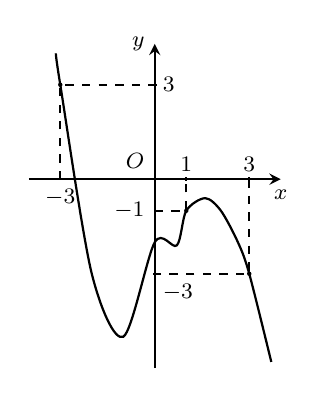
\begin{tikzpicture}[>=stealth,x=1.0cm,y=1.0cm,scale=0.4,thick]
            %\draw [color=gray,dash pattern=on 0.7pt off 1pt,xstep=1.0cm,ystep=1.0cm] (-4.5,-6.5) grid (4.5,4.5);
            \draw[->] (-4,0) -- (4,0) node[below] {\footnotesize $x$};
            \draw[->] (0,-6) -- (0,4.3) node[left] {\footnotesize $y$};
            \foreach \x in {1,3}
            \draw[shift={(\x,0)},color=black] (0pt,2pt) -- (0pt,-2pt) node[above] {\footnotesize $\x$};
            \foreach \y in {-3}
            \draw[shift={(0,\y)},color=black] (2pt,0pt) -- (-2pt,0pt) node[below right] {\footnotesize $\y$};
            \foreach \y in {3}
            \draw[shift={(0,\y)},color=black] (2pt,0pt) -- (-2pt,0pt) node[right] {\footnotesize $\y$};
            \draw (0,0) node[above left] {\footnotesize $O$} (-3,0) node[below] {\footnotesize $-3$} (0,-1) node[left] {\footnotesize $-1$};
            \draw plot[smooth] coordinates {(-3.14,4) (-3,3) (-2,-3) (-1,-5) (0,-2) (0.7,-2.1) (1,-1) (1.6,-.6) (2.1,-1) (2.64,-2) (3,-3) (3.7,-5.8)};
            \draw[dashed] (-3,0) -- (-3,3) -- (0,3) (0,-1)--(1,-1)--(1,0) (3,0)--(3,-3)--(0,-3);
            \fill[black] (-3,3) circle[radius=2pt] (1,-1) circle[radius=2pt] (3,-3) circle[radius=2pt];
        \end{tikzpicture}
    }
    \loigiai{
        \immini{
            Đặt	$g(x)=2f(x)+x^2$.\\
            Ta có $g'(x)=2f'(x)+2x=0\Leftrightarrow f'(x)=-x$.\\
            Từ hình bên suy ra $g'(x)=0$ tại $x=-3,$ $x=1$ hoặc $x=3$.\\
            Hơn nữa, trong khoảng $(-3;1)$ đồ thị $y=f'(x)$ nằm dưới đồ thị $y=-x$ nên $g'(x)$ âm trong khoảng $(-3;1)$.\\
            Xét tương tự trong khoảng $(1;3)$, ta được bảng biến thiên của $g(x)$ như sau.
            \begin{center}
                
\begin{tikzpicture}[>=stealth]
                    \tkzTabInit[nocadre=false,lgt=1,espcl=2,deltacl=0.5]
                    {$x$/.7 ,$y'$/.7,$y$/2}
                    {$-\infty$ , $-3$ , $1$ , $3$ , $+\infty$}
                    \tkzTabLine{ , - , $0$ , + , $0$ , - , $0$ , + , }
                    \tkzTabVar{+/$ $ , -/$ $, +/$ $ , -/$ $ , +/$ $}
                \end{tikzpicture}
            \end{center}
        }{
            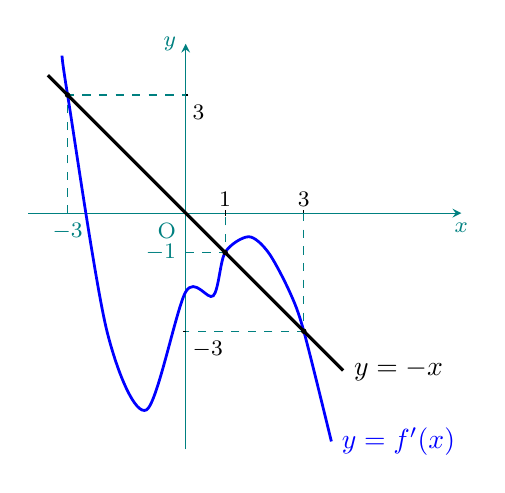
\begin{tikzpicture}[color=teal,>=stealth,x=1.0cm,y=1.0cm,scale=0.5]
                %\draw [color=gray,dash pattern=on 1pt off 1pt,xstep=1.0cm,ystep=1.0cm] (-4.5,-6.5) grid (7.5,4.5);
                \draw[->] (-4,0) -- (7,0) node[below] {\footnotesize $x$};
                \draw[->] (0,-6) -- (0,4.3) node[left] {\footnotesize $y$};
                \foreach \x in {1,3}
                \draw[shift={(\x,0)},color=black] (0pt,2pt) -- (0pt,-2pt) node[above] {\footnotesize $\x$};
                \foreach \y in {-3,3}
                \draw[shift={(0,\y)},color=black] (2pt,0pt) -- (-2pt,0pt) node[below right] {\footnotesize $\y$};
                \draw (0,0) node[below left] {\footnotesize O} (-3,0) node[below] {\footnotesize $-3$} (0,-1) node[left] {\footnotesize $-1$};
                \draw[line width=1.0pt,color=blue] plot[smooth] coordinates {(-3.14,4) (-3,3) (-2,-3) (-1,-5) (0,-2) (0.7,-2.1) (1,-1) (1.6,-.6) (2.1,-1) (2.64,-2) (3,-3) (3.7,-5.8)} node[right]{$y=f'(x)$};
                \draw[dashed] (-3,0) -- (-3,3) -- (0,3) (0,-1)--(1,-1)--(1,0) (3,0)--(3,-3)--(0,-3) ;
                \fill[black] (-3,3) circle[radius=2pt] (1,-1) circle[radius=2pt] (3,-3) circle[radius=2pt];
                \draw[very thick,black,smooth,samples=100,domain=-3.5:4] plot(\x,{-(\x)}) node[right]{$y=-x$};
            \end{tikzpicture}
        }
        \noindent
        Vậy hàm số đồng biến trên khoảng $(-3;1)$ và $(3;+\infty)$.
    }
\end{ex}
%%=====Câu 68
\begin{ex}%[2D1G1-2]
    \immini
    {	Cho hàm số $y=f(x)$ và đồ thị của hàm số $y=f'(x)$ như hình bên dưới. Khi đó hàm số $y=3f(x)-x^3$ đồng biến trên khoảng
        \choice
        {$(0;2)$}
        {$(-2;2)$}
        {$(1;2)$}
        {\True $(-2;1)$}
    }
    {
        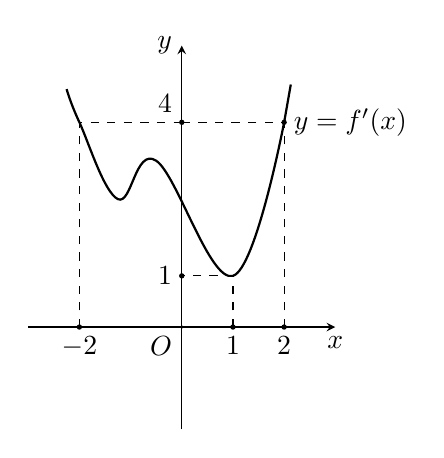
\begin{tikzpicture}[>=stealth,x=1cm,y=1cm,scale=.65]
            \draw[->] (-3,0) -- (3,0) node[below] {$x$};
            \draw[->] (0,-2) -- (0,5.5) node[left] {$y$};
            \draw[thick] plot[smooth,tension=.65] coordinates{(-2.25,4.65) (-2,4) (-1.25,2.5) (-.5,3.25) (1,1) (2,4) }--++(80:0.75);
            \fill (0,0) circle (1pt) node[below left]{$O$};
            \draw[dashed] (-2,0)--(-2,4)--(0,4) (1,0)--(1,1)--(0,1) (2,0)--(2,4)--(0,4);
            \fill (1,0) circle (1.5pt) node[below]{$1$};
            \fill (2,0) circle (1.5pt) node[below]{$2$};
            \fill (-2,0) circle (1.5pt) node[below]{$-2$};
            \fill (0,1) circle (1.5pt) node[left]{$1$};
            \fill (0,4) circle (1.5pt) node[above left]{$4$};
            \fill (2,4) circle (1.5pt) node[right]{$y=f'(x)$};
        \end{tikzpicture}
    }
    \loigiai{
        \immini{
            Đặt $g(x)=3f(x)-x^3$.\\
            Ta có $g'(x)=3f'(x)-3x^2=0\Leftrightarrow f'(x)=x^2$.\\
            Từ hình bên suy ra $g'(x)=0$ tại $x=-2$, $x=1$ hoặc $x=2$.\\
            Hơn nữa, trong khoảng $(-2;1)$ đồ thị $y=f'(x)$ nằm trên đồ thị $y=x^2$ nên $g'(x)>0$ trong khoảng $(-3;1)$.\\
            Xét tương tự trong khoảng $(1;2)$, ta được bảng biến thiên của $g(x)$ như sau.
            \begin{center}
                
\begin{tikzpicture}[color=teal,>=stealth]
                    \tkzTabInit[nocadre=false,lgt=1,espcl=2,deltacl=0.5]
                    {$x$/.7 ,$y'$/.7,$y$/2}
                    {$-\infty$ , $-2$ , $1$ , $2$ , $+\infty$}
                    \tkzTabLine{ , - , $0$ , + , $0$ , - , $0$ , + , }
                    \tkzTabVar{+/$ $ , -/$ $, +/$ $ , -/$ $ , +/$ $}
                \end{tikzpicture}
            \end{center}
        }{
            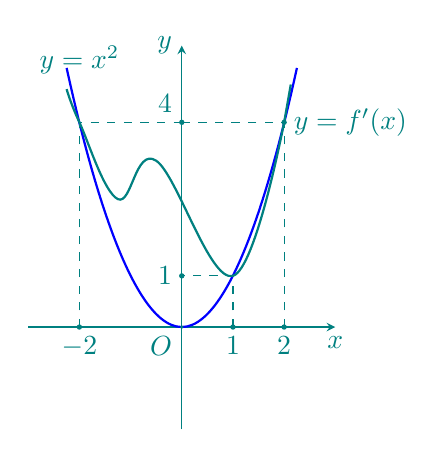
\begin{tikzpicture}[color=teal,>=stealth,x=1cm,y=1cm,scale=.65]
                \draw[->] (-3,0) -- (3,0) node[below] {$x$};
                \draw[->] (0,-2) -- (0,5.5) node[left] {$y$};
                \draw[blue,thick] (-2.25,5.0625) parabola bend (0,0) (2.25,5.0625);
                \draw[thick] plot[smooth,tension=.65] coordinates{(-2.25,4.65) (-2,4) (-1.25,2.5) (-.5,3.25) (1,1) (2,4) }--++(80:0.75);
                \fill (0,0) circle (1pt) node[below left]{$O$};
                \draw[dashed] (-2,0)--(-2,4)--(0,4) (1,0)--(1,1)--(0,1) (2,0)--(2,4)--(0,4);
                \fill (1,0) circle (1.5pt) node[below]{$1$};
                \fill (2,0) circle (1.5pt) node[below]{$2$};
                \fill (-2,0) circle (1.5pt) node[below]{$-2$};
                \fill (0,1) circle (1.5pt) node[left]{$1$};
                \fill (0,4) circle (1.5pt) node[above left]{$4$};
                \fill (2,4) circle (1.5pt) node[right]{$y=f'(x)$};
                \draw (-2,4.75) node[above]{$y=x^2$};
            \end{tikzpicture}
        }
        \noindent
        Vậy hàm số đồng biến trên khoảng $(-2;1)$ và $(2;+\infty)$.
    }
\end{ex}
\begin{ex}%[2D1G1-3]
    Cho hàm số $y=f(x)$ có bảng biến thiên như hình vẽ bên dưới. Tìm tất cả các giá trị của tham số $m$ để hàm số $y=f(\sin 2x-m)$ nghịch biến trên khoảng $\left(\dfrac{3\pi}{4};\pi\right)$.
    \begin{center}
        
\begin{tikzpicture}
            \tkzTabInit[lgt=1.5,espcl=2.5,deltacl=.5]
            {$x$ /.7, $f'(x)$ /.7}
            {$-\infty$,$0$,$3$,$+\infty$}
            \tkzTabLine{,-,$0$,+,$0$,-,}
            %\tkzTabVar{+/$+\infty$,-/$-3$,+/$-\infty$}
        \end{tikzpicture}
    \end{center}
    \choice
    {\True $-3\leq m\leq -1$}
    {$-2\leq m\leq -1$}
    {$-3\leq m\leq 0$}
    {$-2\leq m\leq 0$}
    \loigiai{
        Đặt $t=\sin 2x -m , x\in \left(\dfrac{3\pi}{4};\pi \right) \Rightarrow t\in (-1-m;-m)$ và $t'=2\cos 2x > 0, \forall x\in \left(\dfrac{3\pi}{4};\pi \right)$.
        \\
        $f(\sin 2x+m)$ nghịch biến trên khoảng $\left(\dfrac{3\pi}{4};\pi \right)$
        \\
        $\Leftrightarrow$ $f(t)$ nghịch biến trên khoảng $(-1-m;-m)$
        \\
        $\Leftrightarrow f'(t)\leq 0$
        $\Leftrightarrow \heva{&-1-m\geq 0\\&-m\leq3} \Leftrightarrow -3\leq m\leq -1$.
    }
\end{ex}
\begin{ex}%[2D1G1-3]
    Cho hàm số $f(x)=|x^2-2mx+m+2|$. Có bao nhiêu giá trị nguyên của tham số $m$ thuộc $[-9;9]$ để hàm số đồng biến trên $(0;2)$?
    \choice
    {\True $3$}
    {$2$}
    {$16$}
    {$9$}
    \loigiai{
        $f(x)=|x^2-2mx+m+2| \Rightarrow f'(x)=\dfrac{(2x-2m)(x^2-2mx+m+2)}{|x^2-2mx+m+2|}$.
        \\
        $f'(x) $ đồng biến trên khoảng $(0;2)$ khi $f'(x) \geq 0, \forall x\in (0;2)$
        \\
        $\Leftrightarrow (2x-2m)(x^2-2mx+m+2) \geq 0, \forall x\in (0;2)$.
        \\
        Ta có bảng xét dấu
        \begin{center}
            
\begin{tikzpicture}
                \tkzTabInit[lgt=1.5,espcl=3,deltacl=.5]
                {$x$ /.7, $f'(x)$ /.7}
                {,$m-\sqrt{m^2-m-2}$,$m$,$m+\sqrt{m^2-m-2}$,}
                \tkzTabLine{,-,$0$,+,$0$,-,$0$,+,}
                %\tkzTabVar{+/$+\infty$,-/$-3$,+/$-\infty$}
            \end{tikzpicture}
        \end{center}
        TH1: $m+\sqrt{m^2-m-2}<0 \Leftrightarrow \heva{&m\geq -2\\&m\leq 0} \Rightarrow m=-2;-1;0$.
        \\
        TH2: $\heva{&m-\sqrt{m^2-m-2}\leq 0\\&m\geq 2} \Leftrightarrow \heva{&m\leq -2\\&m\geq 2}$ (vô lí).
        \\
        Vậy có $3$ giá trị của $m$ thỏa yêu cầu đề bài.
    }
\end{ex}
\begin{ex}%[2D1K1-3]
    \immini{Cho hàm số $y=f(x)$ có $f(0)=0$ và đồ thị của hàm $y=f'(x)$ như hình vẽ. Hàm số $y=|4f(x)+x^2|$ đồng biến trên khoảng nào sau đây?
        \choice
        {\True $(0;4)$}
        {$(-\infty;-2)$}
        {$(4;+\infty)$}
        {$(-2;0)$}}{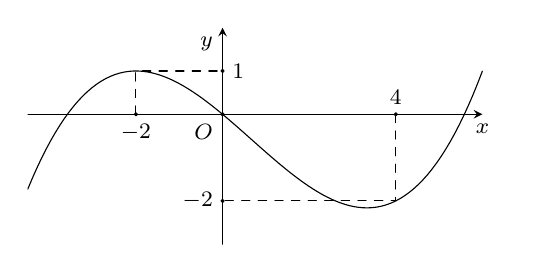
\begin{tikzpicture}[scale=.55, font=\footnotesize, line join=round, line cap=round, >=stealth]
            \def\xmi{-4.5}
            \def\xma{6}
            \def\ymi{-3}
            \def\yma{2}
            \pgfmathsetmacro\hsa{1/24}
            \pgfmathsetmacro\hsb{-1/12}
            \pgfmathsetmacro\hsc{-5/6}
            \clip (\xmi,\ymi) rectangle (\xma+.7,\yma);
            \draw[->] (\xmi,0)--(\xma,0)node[below]{$x$};
            \draw[->] (0,\ymi)--(0,\yma)node[below left]{$y$};
            \draw[dashed] (-2,0)--(-2,1)--(0,1) (4,0)--(4,-2)--(0,-2);
            \foreach \x in {-2,0,4}{
                \draw[fill] (\x,0) circle(1pt);
            }
            \foreach \y in {-2,1}{
                \draw[fill] (0,\y) circle(1pt);
            }
            \draw [domain=\xmi:\xma, samples=100] plot (\x, {\hsa*(\x)^3+\hsb*(\x)^2+\hsc*(\x)});
            \path
            node at (0,1)[right]{$1$}
            node at (4,0)[above]{$4$}
            node at (0,-2)[left]{$-2$}
            node at (0,0)[below left]{$O$}
            node at (-2,0)[below]{$-2$};
        \end{tikzpicture}
    }
\end{ex}
\begin{ex}%[2D1G1-3]
    \immini{Cho hàm số $f(x)$ có đạo hàm trên $\mathbb{R}$ và $f(1)=1$. Đồ thị hàm số $y=f'(x)$ như hình bên. Có bao nhiêu số nguyên dương $a$ để hàm số $y=\left| 4f(\sin x) +\cos2x-a \right|$ nghịch biến trên $\left(0;\dfrac{\pi}{2}\right)$?
        \choice
        {$2$}
        {\True $3$}
        {Vô số}
        {$5$}}{	\begin{tikzpicture}[>=stealth,x=1cm,y=1cm,scale=.8]
            \def\a{.5} % Hệ số a phải khác 0
            \def\b{0}
            \def\c{-1.5}
            \def\d{0}
            \clip (-3.5,-2.5)rectangle(3.5,2.5);
            \draw[->] (-3,0) -- (3,0)node[below]{ $x$};
            \draw[->] (0,-2) -- (0,2) node[left] { $y$};
            \draw (-1,0)node[below]{$-1$};
            \draw (1,0) node[above]{$1$};
            \draw (0,0)node[below left]{ $O$};
            \draw[dashed] (-1,0)--(-1,1) (1,0)--(1,-1);
            \draw[thick,samples=150,smooth,domain=-2.1:2.1] plot(\x,{\a*(\x)^3+(\b)*(\x)^2+(\c)*\x+(\d)});
    \end{tikzpicture}}
    \loigiai{
        Đặt $u=4f(\sin x)+\cos 2x-a$.\\
        $u'=4\cos x\left[f'(\sin x)-\sin x\right]$ $\Rightarrow u'<0$ khi $x \in \left(0;\dfrac{\pi}{2}\right)$.\\
        Bảng biến thiên
        
\begin{tikzpicture}[>=stealth]
            \tkzTabInit[nocadre=false,lgt=1,espcl=3,deltacl=0.5]{$x$/.7 ,$y'$/.7,$y$/2}
            {$0$ , $\dfrac{\pi}{2}$}
            \tkzTabLine{ , - , }
            \tkzTabVar{+/$4f(0)+1-a$ , -/$3-a$}
        \end{tikzpicture}
        $|u|$ nghịch biến trên $\left(0;\dfrac{\pi}{2}\right)$ $\Leftrightarrow 3-a \ge 0 \Leftrightarrow a \le 3$.
    }
\end{ex}
\begin{ex}%[2D1G1-3]
    \immini{Cho hàm số bậc năm $y=f(x)$ có đồ thị của đạo hàm như hình vẽ. Biết $f(-3)<0$, hàm số $y=\left|f(-x^4+2x^3-x^2+1)\right|$ đồng biến trên khoảng nào dưới đây
        \choice
        {$(1;2)$}
        {$(-1;0)$}
        {$(0;0,5)$}
        {$(-2;-1)$}}{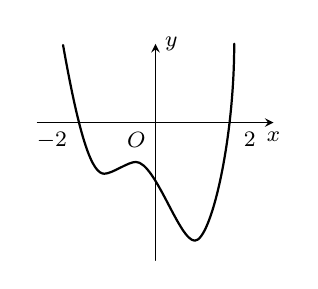
\begin{tikzpicture}[>=stealth, line join=round, line cap=round, font=\footnotesize, scale=.5]
            \draw[<->] (3,0)node[below]{$x$}-|(0,2)node[right]{$y$}
            ;
            \draw (-3,0)-|(0,-3.5) (0,0)node[below left]{$O$};
            \draw[shorten <= -1cm,shorten >= -1cm, thick]
            (-2,0) .. controls +(-80:.5) and +(180:.3) ..
            (-1.3,-1.3) .. controls +(0:.2) and +(180:.2) ..
            (-.5,-1) .. controls +(0:.5) and +(180:.4) ..
            (1,-3) .. controls +(0:.4) and +(-90:.5) ..
            (2,0)
            ;
            \draw (2,0)node[below right]{$2$} (-2,0)node[below left]{$-2$};
    \end{tikzpicture}}
\end{ex}
\Closesolutionfile{ans}
\indapan{10}{ans/2D1-1-DANG-3}